\section{Introduction}

Atom-to-atom mapping assigns corresponding atoms across a reaction. It underlies reaction-center identification, template extraction, and the preparation of endpoint structures for mechanistic calculations. A reaction can admit several plausible correspondences, while many different atom-index assignments are chemically equivalent. An algorithm intended to retain alternatives must therefore resolve two questions: which structural choices deserve separate candidates, and which permutations can be represented together?

Existing approaches use learned correspondence signals or graph-based optimization. RXNMapper derives mappings from attention in a reaction language model~\citep{schwaller2021}; LocalMapper learns from chemist-labeled reactions~\citep{chen2024}; and SLAPMapper combines iterative label refinement with sequential linear assignment~\citep{koda2025}. The Golden benchmark provides a common set of annotated reactions for assessing mapping recovery~\citep{lin2022}. For applications requiring alternatives, recovering the annotation somewhere in a returned family is a different objective from producing one correct top-ranked mapping.

Weighted endpoint graphs introduce a further distinction. A permissive matching tolerance can preserve a fragment despite changes in its bond orders, but the corresponding atom shuffles need not preserve the bond events assigned at a finer threshold. Replacing a compressed family by one representative can therefore hide distinct transformations. Likewise, greedily growing one fragment can prevent a neighboring fragment from reaching an alternative assignment.

MAPPA addresses these issues by branching over structural fragment choices while keeping symmetry-related atom bijections compressed (\Cref{fig:algorithm}). Continuous growth and alternative placements determine the structural choices. Default MAPPA uses one seed ordering per cut and the cut sweep. We introduce a cut-sweep strategy that changes the search conditions to counteract greedy fragment commitment; it is part of default MAPPA, and we also apply it to SLAP to test its benefit beyond our fragment search. Its final representation groups unordered matched fragment pairs and retains the allowed mapping alternatives within each group. A constraint-based decoder projects these families onto distinct bond-event patterns. The method searches for structurally compatible alternatives without requiring the reference transformation to minimize the number of bond changes.

\section{Method}


Algorithm~\ref{alg:mappa-overview} connects the fragment-level operations in \Cref{fig:algorithm}. A live branch stores the fragments already placed, their atom assignments, and the compressed choices still allowed by those decisions. Growing and placing the next fragment conditions every later continuation. The matching routine is treated as an operation here; its compatibility tests and symmetry representation are defined below. For bidirectional search, the search phase is applied in each orientation, retaining the orientation of each returned family.

\begin{algorithm}[t]
\caption{MAPPA: from fragment growth to alternative bond-event candidates}
\label{alg:mappa-overview}
\small
\begin{algorithmic}[1]
\REQUIRE Oriented endpoint graphs, seed orders, optional anchors, search budgets
\ENSURE Compressed final branches; optionally, distinct bond-event candidates
\STATE $\mathcal S\gets\varnothing$ \COMMENT{collected terminal branches}
\FORALL{conditions: uncut source graph and each single-edge source mask}
  \FORALL{requested seed orders under this condition}
    \STATE Initialize live branches with the supplied anchors
    \REPEAT
      \FORALL{seeds in the current order}
        \FORALL{live branches eligible to grow from this seed}
          \STATE Grow a fragment to saturation, conditioned on this branch \COMMENT{Fig.~\ref{fig:algorithm}a}
          \IF{no admissible fragment placement is found}
            \STATE Retain this branch for later seeds
          \ELSE
            \STATE Fork one continuation per distinct structural fragment placement
            \STATE Commit each placement; retain its compressed symmetry and constraints
            \STATE Admit the continuations within the branch budget
          \ENDIF
        \ENDFOR
      \ENDFOR
    \UNTIL{all branches are finished or a full pass makes no progress}
    \STATE Add terminal branches and their search-stop status to $\mathcal S$
  \ENDFOR
\ENDFOR
\STATE Group final branches by unordered fragment pairs; retain their family union
\STATE Expose compressed branches with constraints and provenance
\IF{bond-event candidates are requested as separate post-processing}
  \STATE Decode distinct event classes from complete families using the original matrices
  \STATE Report witnesses, supporting families, and completeness status \COMMENT{Fig.~\ref{fig:algorithm}c}
\ENDIF
\end{algorithmic}
\end{algorithm}

The forks in the search phase represent different fragment placements, not one branch for each symmetry-related bijection. The cut sweep changes the conditions of this search; a single mask can expose a mapping with several bond events. Event decoding is a separate operation on the retained output. Search caps are recorded as truncation, not treated as proof that no alternatives exist.

\subsection{Weighted matching and continuous growth}

Let $V_R,V_P$ be the reactant and product atom sets, $Z_R,Z_P$ their element labels, and $W_R,W_P$ their symmetric bond-weight matrices. A partial mapping $m:D\subseteq V_R\rightarrow V_P$ is injective and element compatible. A mapping assigning every source atom is bijective when the endpoint element counts agree. Explicit hydrogen atoms participate in the search. Molecular coordinates can accompany the graphs but do not determine the growth decisions.

The active source graph contains edges with weight at least $b$. Starting from a seed atom, MAPPA grows a connected source fragment $F$ while carrying multiple compatible product placements. A frontier queue prioritizes stronger source edges. To add an unassigned source atom $u$ with product image $v$, a placement must satisfy
\begin{equation}
 Z_R(u)=Z_P(v),\quad v\notin m(D),\quad
 W_P(v,m(r))\geq b,\quad
 |W_R(u,r)-W_P(v,m(r))|\leq\tau_{\mathrm{iso}}
 \label{eq:match}
\end{equation}
for every active, nonrelaxed source edge $(u,r)$ into $F$. Injectivity is enforced against all current assignments in $D$, including established fragments. All relevant fragment bonds are checked, rather than only the frontier edge that proposed the extension. Source nonedges do not impose negative matching constraints, so additional product bonds remain possible.

An accepted extension enlarges the fragment and filters its compatible placements. Growth continues even if only one placement remains. An unsupported edge is deferred, and other frontier edges can still be explored. When growth reaches an established fragment, ordinary continuation respects its existing assignments. A fragment saturates when no further admissible extension remains; structurally distinct surviving placements then generate separate continuations for the remaining atoms.

This is a greedy search along each trajectory: an accepted extension can remove placements that would support a different fragment boundary. MAPPA broadens coverage through cut sweeps and seed orderings.

\subsection{Cut sweep to vary greedy fragment boundaries}
\label{sec:cut-sweep}

Our cut-sweep strategy reruns growth under alternative source-edge conditions. In addition to the uncut graph $G_R=(V_R,E_R)$, it searches a graph with one eligible edge $e$ removed, $G_R^{(e)}=(V_R,E_R\setminus\{e\})$, for each edge at or above the cut threshold. The evaluated cut threshold equals the active-graph floor $b=0.2$, and eligible edges include bonds to H. Each subrun retains the atom set and the original endpoint weight matrices.

Removing $e$ changes both growth and matching: the frontier cannot extend along that edge, and its bond-preservation test is omitted from \Cref{eq:match}. An extension accepted in the uncut run may otherwise merge atoms into a fragment and discard alternative placements. Under the cut condition, that growth route is unavailable; a fragment can stop at a different boundary, grow through another route, or leave atoms for a later seed. The missing preservation test also admits placements previously excluded by $e$. Thus the sweep counteracts greedy commitment by changing the conditions under which growth proceeds. It does not force the endpoints of $e$ into different final fragments or require a bond-breaking event: they may reconnect through other source edges, and the final correspondence may preserve their bond.

MAPPA takes the union of the uncut and single-edge subruns before final branch deduplication. The default one-seed mode uses one seed ordering per subrun, so it already includes the full cut sweep. There are $|E_R|+1$ subruns at the evaluated thresholds. A single-edge cut describes the search perturbation, not the number of bond events in a returned mapping. One removed constraint can redirect subsequent fragment growth and placements throughout the reaction, exposing an alternative with several bond formations, cleavages, or bond-order changes. MAPPA therefore need not enumerate combinations of final bond events to discover multi-event alternatives. Bond-event decoding uses the original matrices, so a search cut itself contributes no event or event-count penalty. Growth remains greedy within each conditioned subrun; the union broadens coverage without making the search exhaustive.

\begin{figure}[t]
\centering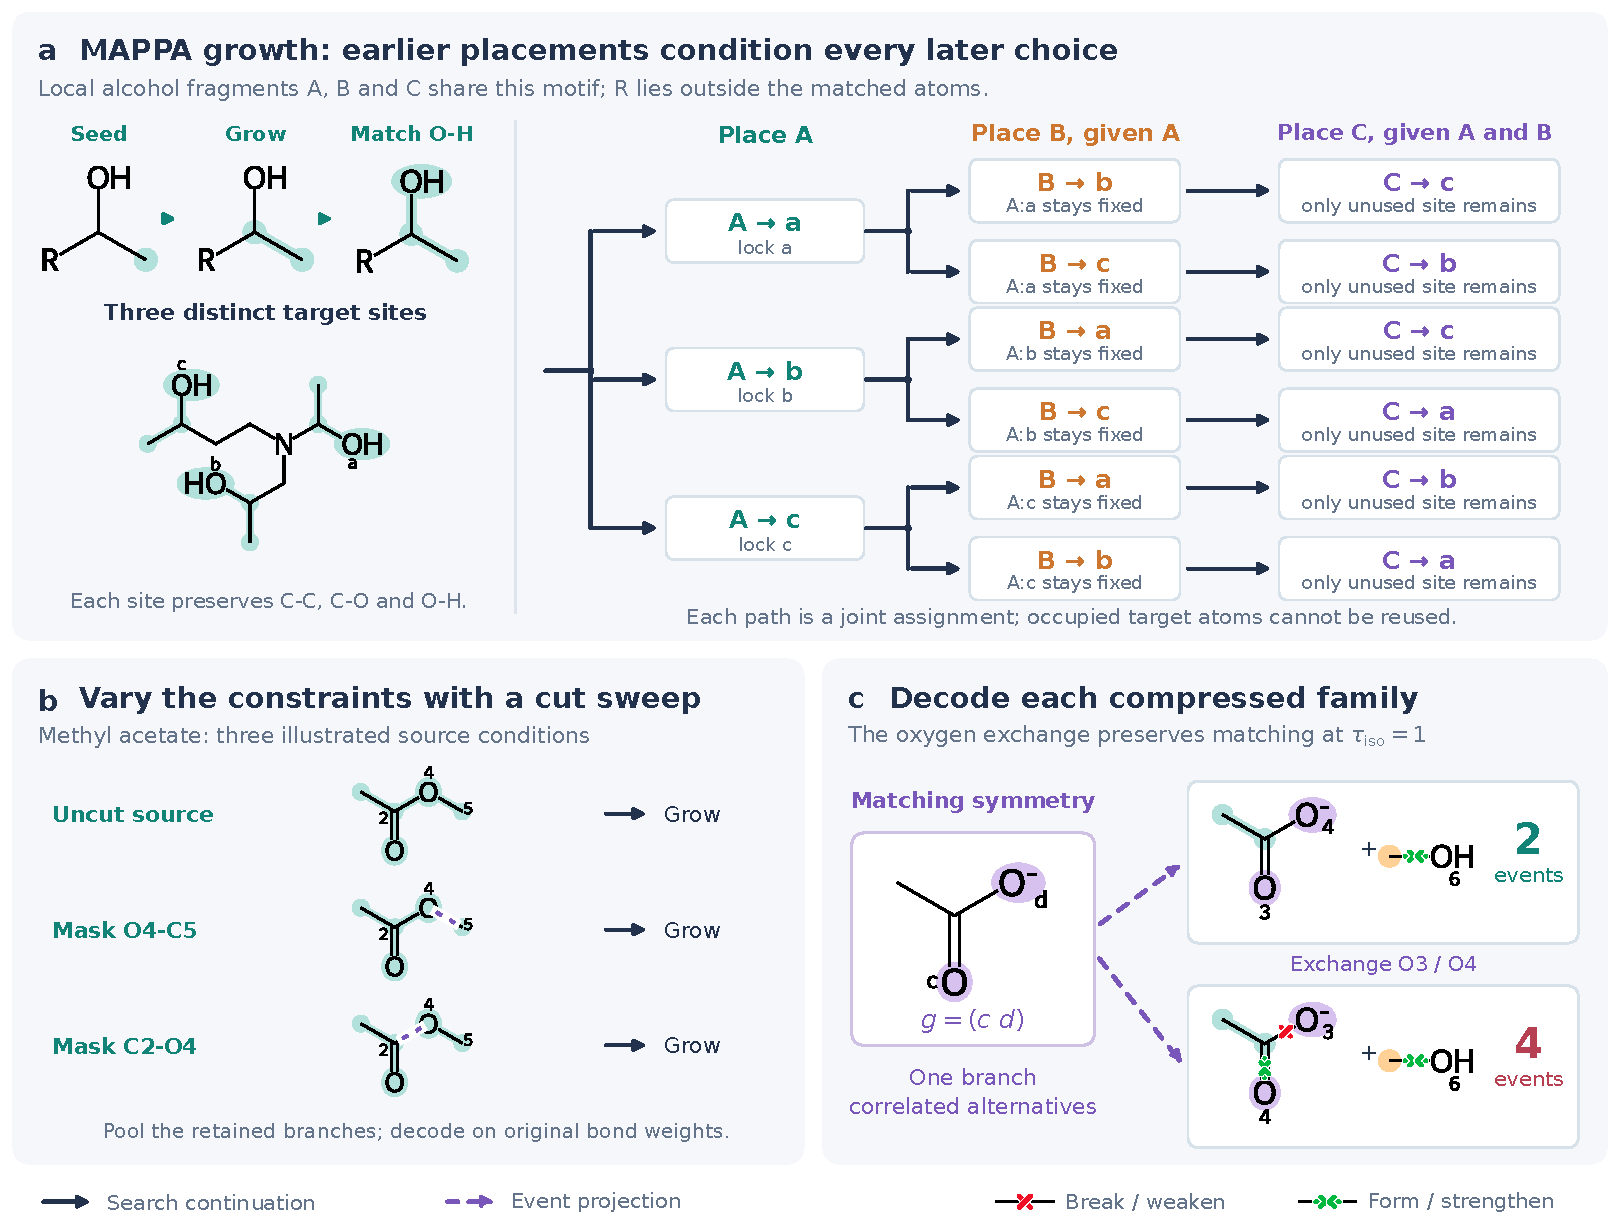
\includegraphics[width=\linewidth]{figs/fig1_algorithm.pdf}
\caption{\textbf{MAPPA: conditional fragment branching and compressed symmetry.} (a) A local alcohol motif grows while retaining its O--H bond. Three sites in the depicted target have distinct molecular environments. For three source fragments sharing this motif, placing A fixes one site; B then branches over the two unused sites, and C takes the remaining site. The tree illustrates local conditioning and injectivity; R denotes atoms outside the matched subgraph, and this is not a complete reaction-search trajectory. All attached hydrogens in the illustrated local matches are checked. (b) The cut sweep searches the uncut source graph and graphs with one source edge masked. The illustrated ester masks change the growth and preservation constraints; their outputs are pooled. Masking an edge does not itself assign a bond event. (c) Exchanging the two acetate oxygen images preserves the fragment's element and bond-weight matching tests at $\tau_{\mathrm{iso}}=1$, but changes two heavy-atom events into four at threshold $0.5$. Neither acetate oxygen carries H. Solid black lines retain the endpoint bonds. Red $\times$ marks on the bonds indicate cleavage or weakening; paired green arrows pointing inward indicate formation or strengthening. Pastel colors track fragment membership or symmetry sites. Dashed arrows are event projections within a family, not additional search branches. Saved constraints govern allowed symmetry actions. These formal-bond-order event signatures illustrate MAPPA decoding, not distinct mechanisms or resonance-normalized transformations.}
\label{fig:algorithm}
\end{figure}

\begin{samepage}
\subsection{Automorphisms and correlated mapping families}

The distinction between structural branches and explicit bijections is central to the design. Even one fragment family can contain combinatorially many assignments: $k$ independently exchangeable methyl-hydrogen triplets admit $(3!)^k$ bijections. Expanding those automorphisms into separate mappings would multiply the work without adding fragment choices. MAPPA instead stores the permitted permutation actions and their constraints, and decodes event alternatives directly from this representation. Branch caps bound retained alternatives within each growth call; they do not guarantee a small global search. This avoids explicitly listing symmetry-related bijections within each retained family.
\end{samepage}

Compatible placements are stored using a representative assignment, unresolved assignment blocks, and permutation generators. During growth, graph canonicalization accounts for the current fragment, locked assignments, and boundary information. Each saved transition records its action generators together with conditioning and fragment-preservation constraints; their conjunction defines the allowed mapping relation. Canonical labeling and automorphism computation use nauty~\citep{mckay2014}.

Matching tolerance and automorphism equivalence have different roles. The relation $|x-y|\leq\tau_{\mathrm{iso}}$ is generally not transitive, so it does not by itself define a permutation group. To describe an intrinsic symmetry shared by a final fragment pair, we instead color product bonds by their responses to the fragment's matching tests. For a product weight $w$ and the set $\mathcal W$ of active reactant weights for the same element pair, the label records
\begin{equation}
 \chi_{\mathcal W}(w)=\left(\mathbf 1[w\geq b],
 \left(\mathbf 1[w\geq b\ \land\ |w-v|\leq\tau_{\mathrm{iso}}]\right)_{v\in\mathcal W}\right).
 \label{eq:response}
\end{equation}
An exact automorphism of this colored graph preserves every encoded matching test. This definition depends on the final fragment pair, not its growth order.

The saved mapping relation also contains the constraints imposed by its search decisions. We represent a flat family $\mathcal F_j$ by a seed mapping $m_j$, a sequence of allowed action groups $G_{j,1},\ldots,G_{j,k}$, and final preservation constraints $C_j$:
\begin{equation}
 \mathcal F_j=\left\{a_k\circ\cdots\circ a_1\circ m_j:
 a_i\in G_{j,i},\ C_j(a_k\circ\cdots\circ a_1\circ m_j)\right\}.
 \label{eq:family}
\end{equation}
These actions encode correlated moves; atoms in a common orbit are not independently permutable. Disjoint actions commute and can be placed in a canonical order. The order of overlapping actions is retained. A sequence of groups is not generally equivalent to the group generated by their union.

The intrinsic automorphism of a fragment pair is shared metadata, not permission to enlarge its saved family. Multiple admissible seed mappings can occupy different intrinsic symmetry orbits, and different search constraints can restrict the allowed actions. MAPPA therefore retains these alternatives explicitly inside the compressed representation.

\subsection{Unordered final branches}

During search, history and boundary conditions matter because they determine valid continuation. At completion, the branch identity is instead the unordered collection of matched atom sets,
\begin{equation}
 \mathcal B=\{(R_1,P_1),\ldots,(R_q,P_q)\},
 \qquad P_i=m(R_i),
 \label{eq:branch}
\end{equation}
under a fixed matching policy. Sorting atoms within each set and then sorting the fragment pairs removes dependence on growth order and fragment labels. Growing $A$ before $B$ or $B$ before $A$ yields one branch when the final paired sets agree. The colors within each candidate in \Cref{fig:alternatives} illustrate these matched fragment pairs.

Each branch stores the union of its flat families. Identical normalized family records are shared, while distinct constraints or action programs remain available. This transformation preserves the represented mapping union: it changes its grouping, not its admissible assignments. Provenance links retain the discovering paths, but the original search hierarchy is unnecessary for decoding. This conservative deduplication does not assert that the remaining families are mutually disjoint.

\subsection{Decoding distinct bond-event patterns}

For each complete mapping, define the signed change for an unordered source pair $\{u,v\}$ by
\begin{equation}
 \Delta_{uv}(m)=W_P(m(u),m(v))-W_R(u,v),\qquad
 s_{uv}(m)=
 \begin{cases}
 +1,&\Delta_{uv}(m)\geq\delta_{uv},\\
 -1,&\Delta_{uv}(m)\leq-\delta_{uv},\\
 0,&\text{otherwise}.
 \end{cases}
 \label{eq:events}
\end{equation}
Positive events denote bond formation or strengthening; negative events denote cleavage or weakening. The event count is $E(m)=\sum_{u<v}\mathbf 1[s_{uv}(m)\ne0]$. The evaluation includes hydrogen atoms and all atom pairs. For the WBO collection, $\delta_{uv}=0.3$ for pairs involving a metal and $0.5$ otherwise. These thresholds are independent of $\tau_{\mathrm{iso}}$. \Cref{fig:alternatives} provides a concrete example: changing the atom correspondence changes which pairs gain or lose bond order, even when the total event counts agree (A and C).

The decoder returns one bijection witness per distinct signed event class, identifying patterns related by exact source permutations that preserve all thresholded bond-change tests. Matching-preserving shuffles can therefore yield different event classes. The decoder first certifies families whose assignments all yield equivalent events and excludes families outside the requested event window. It then encodes the remaining family constraints symbolically in Z3~\citep{demoura2008}. Each solution supplies a witness and its event pattern; excluding that entire event class allows the next distinct pattern to be found. This avoids enumerating individual bijections or permutation groups.

For a window $E\leq K$, decoding is complete when every retained family is certified exhausted or excluded. A timeout leaves completeness unresolved. This certificate concerns the saved search output within the window; it does not establish exhaustive exploration of all chemically possible mappings. The default deduplication preserves families that contain different event counts, as illustrated in the heavy-atom projection in \Cref{fig:algorithm}c.

\FloatBarrier
\subsection{Alternative correspondences and chemical interpretation}

An atom mapping summarizes the net correspondence resulting from a chemical process without specifying its intermediates or elementary steps. When that pathway is unknown, endpoint structures alone may not determine a unique correspondence. MAPPA therefore retains alternative bond-event patterns and the correlated shuffles within each, exposing one witness per event class together with its supporting families and conditional symmetry queries. Distinct patterns can have equal event counts, and minimizing the count need not recover the reference correspondence.

\Cref{fig:alternatives} illustrates both points with Golden case 9. MAPPA recovers the annotated correspondence, in which the alcohol oxygen enters the product ring and the ketone oxygen leaves in water (A). Another candidate exchanges these oxygen origins (B); a third also exchanges two carbon assignments (C). Candidate B has fewer total events than the reference, while A and C have equal totals but different correspondences. Thus, selecting either one bijection or only the lowest event count discards information about the alternatives. These are selected witnesses from the search, not an exhaustive decoded set or validated reaction pathways.

\begin{figure}[t]
\centering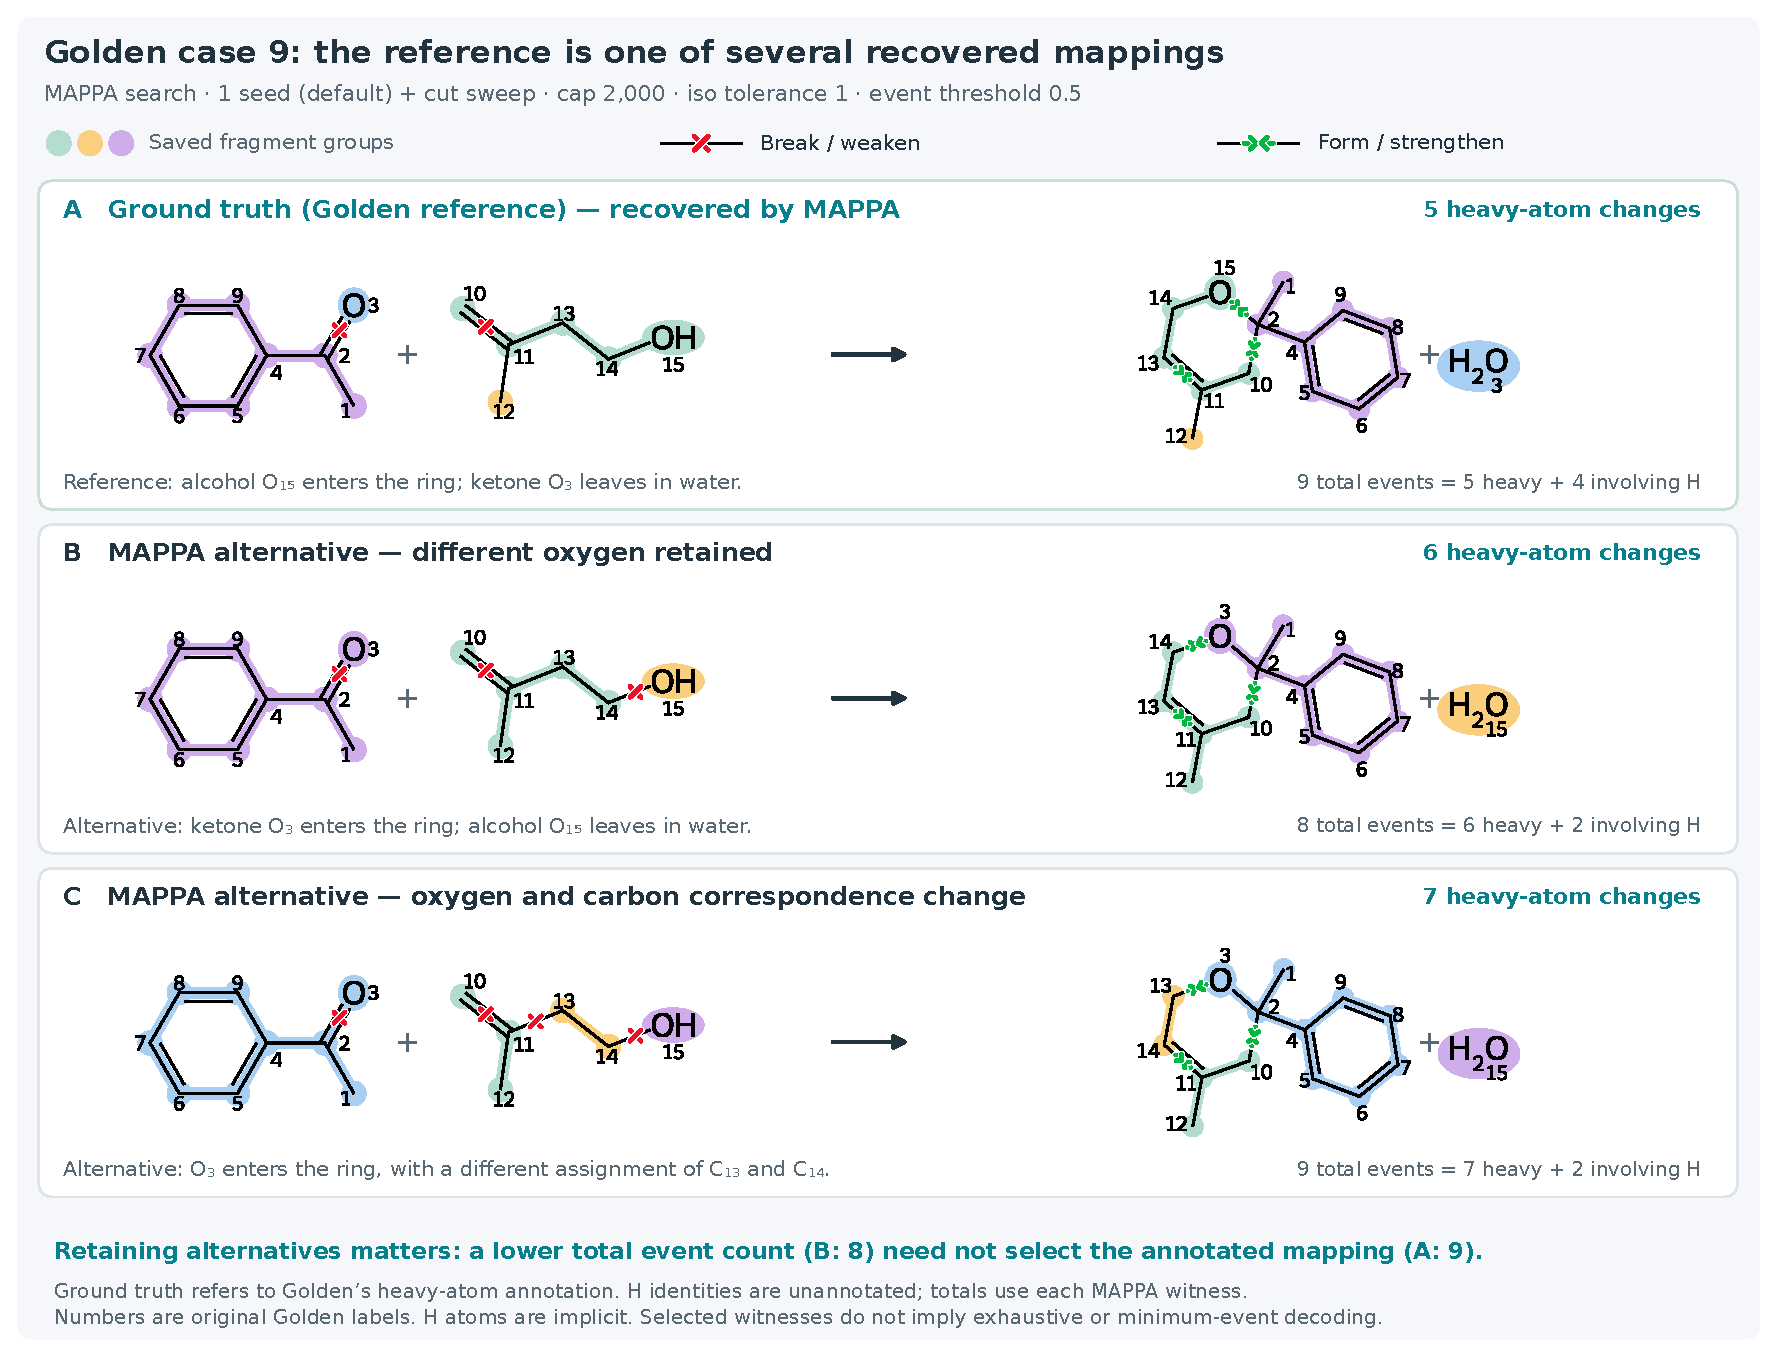
\includegraphics[width=\linewidth]{figs/fig4_alternatives.pdf}
\caption{\textbf{A recovered reference and alternative correspondences from Golden case 9.} A matches all 15 annotated heavy-atom pairs. B exchanges the oxygen origins; C also exchanges C$_{13}$/C$_{14}$. Pastel colors identify matched fragments. Black lines show endpoint bonds; red $\times$ marks indicate cleavage or weakening, and green inward arrows indicate formation or strengthening. H atoms are implicit in the drawing; event totals include H. Each witness minimizes H-involving changes for its fixed heavy-atom correspondence. ``Ground truth'' denotes the dataset annotation, not a verified pathway. The three witnesses come from one-seed MAPPA sweep search at cap 2,000 and $\tau_{\mathrm{iso}}=1$, without reference labels; events use threshold 0.5.}
\label{fig:alternatives}
\end{figure}

\FloatBarrier
\section{Evaluation}

\subsection{Datasets and comparison protocol}

We evaluate reference recovery on all 1,851 Golden reactions~\citep{lin2022} and bond-event alternatives on 140 coordinate/WBO endpoint pairs. Golden inputs use formal bond orders and explicit H, with reference labels removed before search. Recovery requires the annotated heavy-atom correspondence, including unmatched atoms, modulo endpoint chemical symmetries preserving charge, isotope, H count, and stereochemistry. Failures and unresolved cases remain in the denominator. This measures reference inclusion among returned alternatives, not their ranking.

LocalMapper provides the prior accuracy-SOTA baseline~\citep{chen2024}. Its published Golden accuracy was 89.8\% on 1,758 retained reactions with manual calibration. SLAP reported 86.9\% on that dataset version, counting reference inclusion among its candidates~\citep{koda2025}. These literature scores are separate from our strict re-evaluation. We additionally apply the cut sweep introduced here to SLAP; ``SLAP sweep'' denotes this extension, not a published SLAP score. It is our strongest evaluated prior-method baseline for alternative recovery. Released RXNMapper, Chython, Indigo, and RDT provide further comparisons~\citep{schwaller2021,chython,indigo,rahman2016}.

The coordinate collection contains 18--137 explicit atoms per endpoint, including organometallic and multicomponent structures. It was inspected during development and has no verified atom mappings: it is not a mapping-accuracy benchmark. We compare the lowest event count found and the patterns achieving that count. MAPPA uses supplied WBO matrices; SLAP uses XYZ-derived binary graphs. Returned SLAP heavy-atom assignments receive hydrogen refinement and are then scored on the same WBO matrices as MAPPA using \Cref{eq:events}. The comparison covers those witnesses, not all possible SLAP hydrogen assignments.

\begin{table}[tb]
\centering\small
\caption{\textbf{Evaluation configurations.} Both use $b=0.2$, $\tau_{\mathrm{iso}}=1$, explicit H, and uncut plus single-edge searches. Default MAPPA uses one seed per cut, the sweep. Golden measures the sweep-search stage; no-sweep controls retain only the uncut graph. A seed setting counts source-atom orderings per cut.}
\label{tab:protocol}
\begin{tabular}{lcc}\toprule
Setting & Golden & Coordinate/WBO\\\midrule
Reactions & 1,851 & 140\\
Search directions & Bidirectional & Reactant to product\\
Seed orderings & 1 (default), 2, 3, 10 & 1 (default)\\
Branch cap & 100 (default) & 100 (default), 2,000\\
Evaluation & Reference-family recovery & Signed event-class coverage\\\bottomrule
\end{tabular}
\end{table}

\Cref{tab:protocol} lists the evaluated settings. Search does not use reference or comparator correspondences. Full configurations, implementation versions, and reproduction scripts are provided in the repository (\Cref{sec:reproducibility}).

\subsection{Golden reference recovery and search cost}

Default MAPPA recovers \GoldenOnePercent\% of Golden references, compared with \SlapPercent\% for SLAP sweep (\Cref{tab:competitors,fig:golden}). The paired comparison includes \AamOnly{} references recovered only by MAPPA and \SlapOnly{} only by SLAP. LocalMapper is the strongest evaluated method returning one bijection. Additional MAPPA seeds yield modest recovery gains at increasing search cost; two seeds do not improve recovery over the default.

\begin{table}[tb]
\centering\small
\setlength{\tabcolsep}{4pt}
\caption{\textbf{Golden reference recovery and runtime.} Recovery uses all 1,851 primary-evaluation records. MAPPA retains compressed families; SLAP returns explicit candidates; other methods return one bijection over their matched atoms. MAPPA uses cap 100 and bidirectional search. Bidirectional SLAP combines both directions and both binary/weighted modes; the default SLAP row uses binary only. Times are mean CPU seconds per reaction, excluding separate bond-event decoding. Unmarked times use the same 1,403 completed reactions on an AMD EPYC 9J14. $a$: archived completed calls (1,718--1,851 per method), CPU model unrecorded; these times are not directly comparable with unmarked times. $\dagger$: LocalMapper, prior accuracy SOTA (2024). $\ddagger$: SLAP with our sweep, strongest evaluated prior-method recovery baseline.}
\label{tab:competitors}
\begin{tabular}{@{}lllr r@{}}\toprule
Method & Search setting & Output & Reference recovered & Mean CPU s\\\midrule
MAPPA & 1 seed, sweep (default) & Families & 1,834 (99.08\%) & 0.963 \\
MAPPA & 2 seeds, sweep & Families & 1,834 (99.08\%) & 1.619 \\
MAPPA & 3 seeds, sweep & Families & 1,837 (99.24\%) & 2.265 \\
MAPPA & 10 seeds, sweep & Families & 1,840 (99.41\%) & 6.993 \\
MAPPA & 1 seed, no sweep & Families & 1,489 (80.44\%) & 0.040 \\
SLAP, bidirectional & No sweep & Candidates & 1,661 (89.74\%) & 0.105 \\
SLAP, bidirectional$^{\ddagger}$ & Sweep & Candidates & 1,796 (97.03\%) & 2.793 \\
SLAP, binary & Default, no sweep & Candidates & 1,591 (85.95\%) & 0.075$^{a}$ \\
RXNMapper & Default, no sweep & One bijection & 1,547 (83.58\%) & 0.056$^{a}$ \\
LocalMapper$^{\dagger}$ & Default, no sweep & One bijection & 1,605 (86.71\%) & 0.294$^{a}$ \\
Chython & Default, no sweep & One bijection & 1,561 (84.33\%) & 0.612$^{a}$ \\
Indigo & Default, no sweep & One bijection & 692 (37.39\%) & 0.184$^{a}$ \\
RDT & Default, no sweep & One bijection & 1,030 (55.65\%) & 1.021$^{a}$ \\
\bottomrule\end{tabular}

\end{table}

The cut sweep is central to this result: it adds 345 reference recoveries for MAPPA and 135 for SLAP. Without the sweep, one-seed MAPPA has lower coverage than bidirectional SLAP. This supports varying the growth constraints to expose alternatives excluded by greedy fragment extension (\Cref{sec:cut-sweep}); symmetry expansion alone cannot restore discarded placements.

Smaller-first grows fragments from the reaction side with fewer explicit atoms (including H) and matches into the other side; larger-first reverses these roles. Bidirectional search combines both outputs. It adds 31 recoveries over smaller-first alone, demonstrating that the two orientations retain complementary alternatives (\Cref{tab:directions}).

\begin{table}[tb]
\centering\small
\caption{\textbf{Recovery and runtime by search orientation.} All rows use the sweep. Recovery uses all 1,851 Golden records; CPU statistics are seconds per reaction over the same \CommonCases{} completed reactions (Apple M4 Pro CPU). Smaller-first grows from the side with fewer explicit atoms, including H; larger-first reverses the source and target. Equal-size ties use stored order and its reverse. Bidirectional output combines both searches, and its CPU cost is their sum. SLAP combines binary and weighted modes. CPU/SLAP compares means within each orientation. Timing scopes are specified in \Cref{sec:reproducibility}.}
\label{tab:directions}
\begin{tabular}{@{}llrrrrr@{}}\toprule
Method & Orientation & Recovered & Mean & Median & 95th pct. & CPU/SLAP\\\midrule
MAPPA, 1 seed (default) & Smaller-first & 1,803 (97.41\%) & 1.141 & 0.263 & 5.289 & 0.34\\
 & Larger-first & 1,779 (96.11\%) & 1.377 & 0.348 & 6.401 & 0.92\\
 & Bidirectional & 1,834 (99.08\%) & 2.518 & 0.719 & 12.913 & 0.52\\
\midrule
MAPPA, 2 seeds & Smaller-first & 1,815 (98.06\%) & 2.232 & 0.416 & 10.635 & 0.67\\
 & Larger-first & 1,805 (97.51\%) & 2.721 & 0.578 & 14.064 & 1.83\\
 & Bidirectional & 1,834 (99.08\%) & 4.953 & 1.250 & 26.350 & 1.03\\
\midrule
SLAP sweep (prior baseline) & Smaller-first & 1,775 (95.89\%) & 3.329 & 0.422 & 4.752 & 1.00\\
 & Larger-first & 1,770 (95.62\%) & 1.490 & 0.455 & 4.568 & 1.00\\
 & Bidirectional & 1,796 (97.03\%) & 4.819 & 0.881 & 11.048 & 1.00\\
\bottomrule\end{tabular}

\end{table}

Default MAPPA has a lower mean and median search cost than SLAP sweep, but a higher 95th percentile. Two seeds approximately double the mean cost without improving recovery here. Golden timings cover search, excluding reference verification and separate bond-event decoding. The two timing tables use different experiments and should be compared within their stated CPU and reaction sets.

Increasing the branch cap from 100 to 2,000 yields no additional swept recoveries among cases resolved at both caps, while increasing cost and unresolved outcomes at higher seed counts (\Cref{tab:golden-caps}). The uncut search gains 19 confirmed recoveries. Thus, a larger branch budget does not substitute for changing the growth conditions.

The default-comparator rows in \Cref{tab:competitors} use released interfaces without prediction repair or reference-guided reranking. Binary SLAP is retained as the stronger default configuration. The other methods return at most one explicit bijection per reaction, whereas SLAP returns multiple candidates. Invalid endpoint chemistry and duplicate atom labels count as failures; the repository records their frequencies. These results describe the evaluated interfaces and scoring rule, including its difference from RDT's chemical-change criterion.

\begin{figure}[tb]
\centering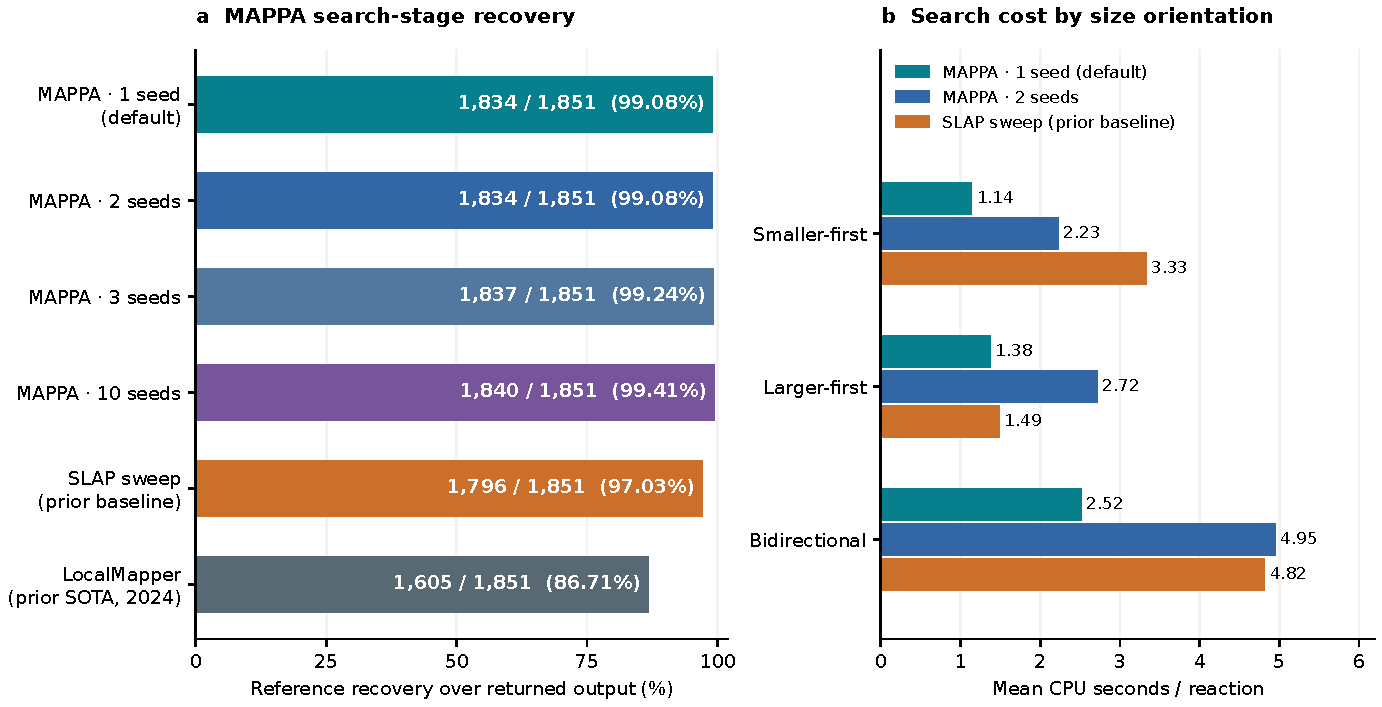
\includegraphics[width=\linewidth]{figs/fig2_golden.pdf}
\caption{\textbf{Golden reference recovery and search cost.} (a) Reference recovery over all 1,851 reactions. MAPPA and SLAP use our cut sweep; LocalMapper is the prior accuracy-SOTA baseline and returns one bijection. All scores use our evaluator. (b) Mean search CPU over the same \CommonCases{} completed reactions, by orientation. Bond-event decoding is excluded. Full comparisons and timing scopes are in \Cref{tab:competitors,tab:directions}.}
\label{fig:golden}
\end{figure}

\FloatBarrier
\subsection{Minimum bond-event comparison on 140 coordinate reactions}

We use one-seed MAPPA sweep search at cap 2,000, which returns complete mappings for all 140 reactions. Cap 100 leaves two reactions incomplete (cases 123 and 125). The larger cap is therefore used for this comparison; the library default remains 100.

MAPPA matches or lowers the minimum event count found by both native SLAP and SLAP sweep in every reaction (\Cref{tab:coordinate-minima,fig:coordinate}). This does not imply recovery of every alternative: at equal minima, six SLAP-sweep patterns remain absent across four reactions. An equal count can describe different changed bonds, and a lower count alone does not establish a more plausible transformation.

\begin{table}[H]
\centering\small
\caption{\textbf{Minimum bond-event comparison on 140 reactions.} MAPPA uses one-seed sweep search at cap 2,000. The first three columns count reactions by MAPPA's minimum event count relative to the comparator. The final column gives comparator minimum-event patterns recovered by MAPPA among reactions with equal minima. Counts refer to returned candidates, not proven global optima.}
\label{tab:coordinate-minima}
\begin{tabular}{@{}lrrrr@{}}\toprule
Compared with & MAPPA fewer & Equal & MAPPA more & Patterns at equal minima\\\midrule
SLAP sweep & 4 & 136 & 0 & 158/164\\
Native SLAP & 15 & 125 & 0 & 138/140\\
\bottomrule\end{tabular}

\end{table}

To compare alternatives above MAPPA's own minima, we decode through one event above the higher of the two SLAP minima for each reaction. MAPPA retains 162 of 168 SLAP-sweep minimum-event patterns and 151 of 160 native-SLAP patterns within these windows. The output contains 300 distinct patterns, including 166 at MAPPA's own minima. Every saved family is decoded or certified within its window; this establishes completeness for the retained families, not exhaustive structural search.

\begin{table}[H]
\centering\small
\caption{\textbf{Stage CPU time per reaction on the 140 coordinate reactions.} Measurements use an Apple M4 Pro CPU. MAPPA uses one-seed sweep search at cap 2,000. These stage costs exclude MAPPA decoding and do not establish an end-to-end speed ranking. SLAP refinement covers its returned witnesses. Timing boundaries are specified in \Cref{sec:reproducibility}.}
\label{tab:coordinate-time}
\begin{tabular}{@{}lrrr@{}}\toprule
Recorded stage & Mean CPU s & Median CPU s & 95th pct. CPU s\\\midrule
MAPPA sweep search & 1.047 & 0.314 & 3.481\\
SLAP sweep mapping & 1.337 & 0.546 & 5.919\\
SLAP H refinement / initial scoring & 0.053 & 0.011 & 0.207\\
\bottomrule\end{tabular}

\end{table}

The stage timings in \Cref{tab:coordinate-time} cover different outputs: MAPPA search retains families for subsequent decoding, while SLAP refinement operates on returned witnesses. They therefore do not establish an end-to-end speed ranking.

\input{includes/generated-end-to-end-text}

\begin{figure}[tb]
\centering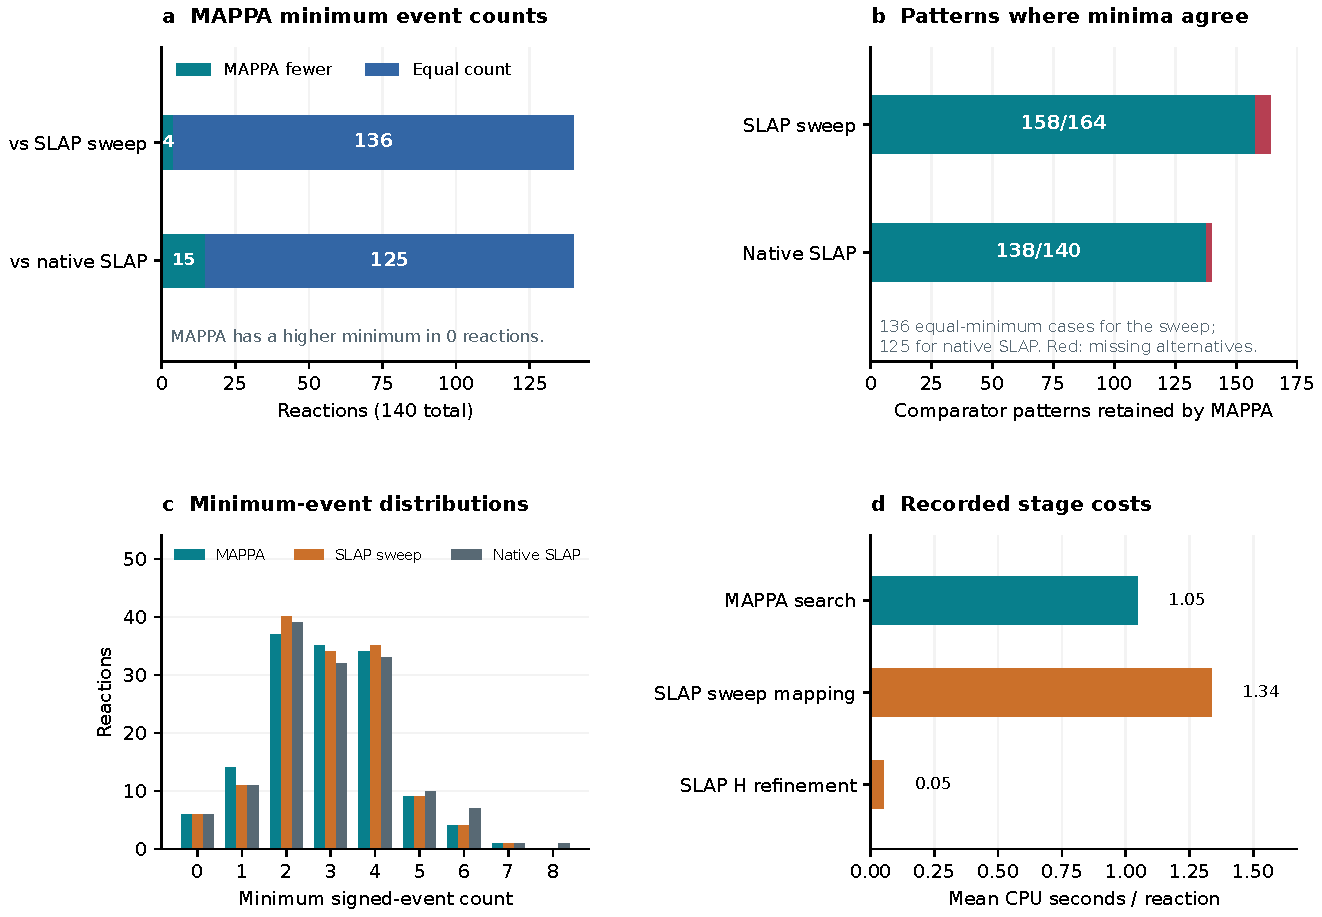
\includegraphics[width=\linewidth]{figs/fig3_coordinate.pdf}
\caption{\textbf{Bond-event comparison on 140 coordinate reactions.} MAPPA uses one seed, the sweep, and cap 2,000. (a) Reactions with fewer or equal MAPPA events than each SLAP baseline. (b) Comparator minimum-event patterns recovered by MAPPA at equal minima. (c) Minimum-event count distributions. (d) Mean CPU for search and SLAP refinement, excluding MAPPA decoding (\Cref{tab:coordinate-time}). Atom mappings are unverified; this compares bond events, not mapping accuracy.}
\label{fig:coordinate}
\end{figure}

\FloatBarrier
\section{Discussion}

\subsection{Applications and future directions}

Atom correspondence is a preprocessing decision in reaction-path interpolation: the assignment determines which product position each reactant atom approaches. Atomic-index assignment is a recognized obstacle in reaction-pathway search~\citep{de2019}. MAPPA's complete correspondences and allowed joint shuffles could be used to reorder and align endpoints before constructing initial paths for nudged elastic band (NEB) calculations~\citep{henkelman2000}. Different event patterns provide alternative reaction cores, while symmetry-related assignments within one pattern can give different interpolations. This offers a systematic way to prepare several TS-search starting points. Mapping the same core into a TS guess also allows its vibrational modes to be assessed against the intended bond changes.

Structure verification is another application. A generative model may return a molecule with reordered atoms or a different conformation, making direct coordinate comparison unsuitable for checking its connectivity. AAM supplies an explicit correspondence under which the target and generated structures can be compared for missing or extra connections. A complete witness that passes this comparison certifies agreement under the chosen graph representation and tolerances. Connectivity alone does not establish stereochemical identity or energetic stability, and failure to find a witness in a bounded search is not proof of a mismatch.

Such checks could also supply a verification mechanism for large language model (LLM) post-training, including reinforcement learning with verifiable rewards (RLVR)~\citep{lambert2024}. For tasks that ask a model to generate a target structure or satisfy specified structural constraints, an independently checked atom correspondence could provide a task-specific reward. The reward would certify the stated structural conditions, with unresolved searches kept distinct from verified failures. This is a proposed use of the verifier; we have not evaluated an RLVR training loop or its effect on molecular generation.

For pathway and retrosynthesis analysis, alternative event patterns expose different atom origins, reaction centers, and possible fragment disconnections. These could help organize mechanistic hypotheses or compare proposed precursors while retaining symmetry-related choices for subsequent geometric analysis. One net correspondence can admit several intermediate sequences, however, and a compatible mapping need not describe a feasible reaction. Energies, reaction conditions, stereochemistry, and experimental evidence remain necessary to assess the proposed routes. The present evaluation concerns correspondence coverage and bond-event alternatives; it does not measure improvements in NEB convergence, TS-search success, or synthesis planning.

Alternative enumeration is not unique to MAPPA or SLAP; for example, an Ising-computing approach enumerates optimal mappings and reduces them by molecular symmetry~\citep{ali2025}. MAPPA's contribution is to retain conditional fragment families and expose their distinct event patterns and allowed shuffles without expanding all bijections.

\FloatBarrier
\subsection{Coverage and remaining search limitations}

An audit of all eleven ten-order Golden misses separates unmatched-atom decisions from fragment-placement failures (\Cref{tab:golden-misses}). In four reactions, every retained family maps exactly one more heavy-atom pair than the reference. Such a family cannot reproduce the reference's unmatched-atom pattern through symmetry shuffling: permutations preserve the number of assigned pairs. The remaining seven lack the required correspondence within their saved families. Re-ranking or expanding those families into explicit bijections cannot supply a missing structural alternative.

Two traced examples show how greedy extension excludes a representable reference. One reference exchanges adjacent labels in an otherwise unchanged pyridine ring; another exchanges the carbonyl-oxygen attachments of oxalic acid across its retained carbons. Ordinary growth preserves bonds that these correspondences require separating. Uncapped trajectories still miss both references, while reference-constrained fragment choices establish their representability. In the oxalic-acid example, a reference-selected three-edge relaxation also exposes the reference to ordinary matching; the single-edge sweep does not contain that cut set. These are feasibility diagnostics, not additional benchmark recoveries. For the other five correspondence misses, the audit does not isolate cap truncation from unsampled growth choices. They motivate selective alternatives to successful growth extensions and explicit choices about leaving atoms unmatched, rather than treating larger caps or more symmetry expansion as sufficient remedies.

Only one of the eleven misses is recovered by any tested comparator configuration, including the SLAP sweep. The shared failures warrant inspection of the supplied correspondences as well as search improvements; they do not establish annotation errors. All eleven remain in the reported denominator. Independent evaluation on annotated coordinate reactions is needed to assess generalization beyond the development collection.
